\documentclass{standalone}
\usepackage{ctex}

\usepackage{tikz}
\usepackage{pgfplots}
\pgfplotsset{compat = newest}
\begin{document}

\begin{tabular}{|c|}

\hline

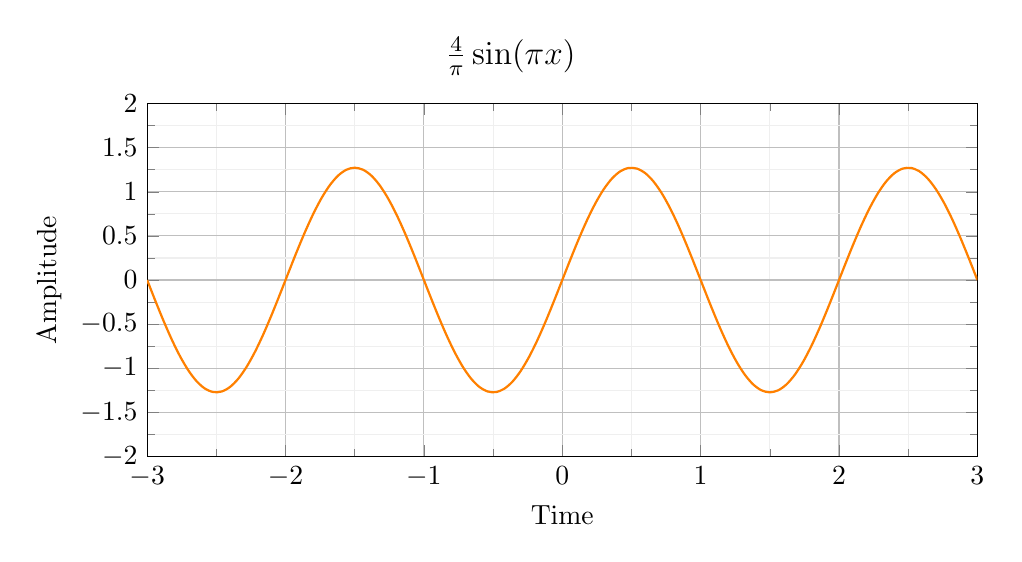
\begin{tikzpicture}
\begin{axis}[
xmin = -3, xmax = 3,
ymin = -2, ymax = 2.0,
xtick distance = 1,
ytick distance = 0.5,
grid = both,
minor tick num = 1,
major grid style = {lightgray},
minor grid style = {lightgray!25},
width = \textwidth,
height = 0.5\textwidth,
xlabel=Time,
ylabel=Amplitude,
trig format plots=rad
]
\addplot[
domain = -3:3,
samples = 101,
smooth,
thick,
orange,
] {(4 / (pi)) * sin(pi * x)};
\end{axis}
\node[above,font=\large\bfseries] at (current bounding box.north) {$\frac{4}{\pi}\sin(\pi x)$};
\end{tikzpicture}

\\\hline

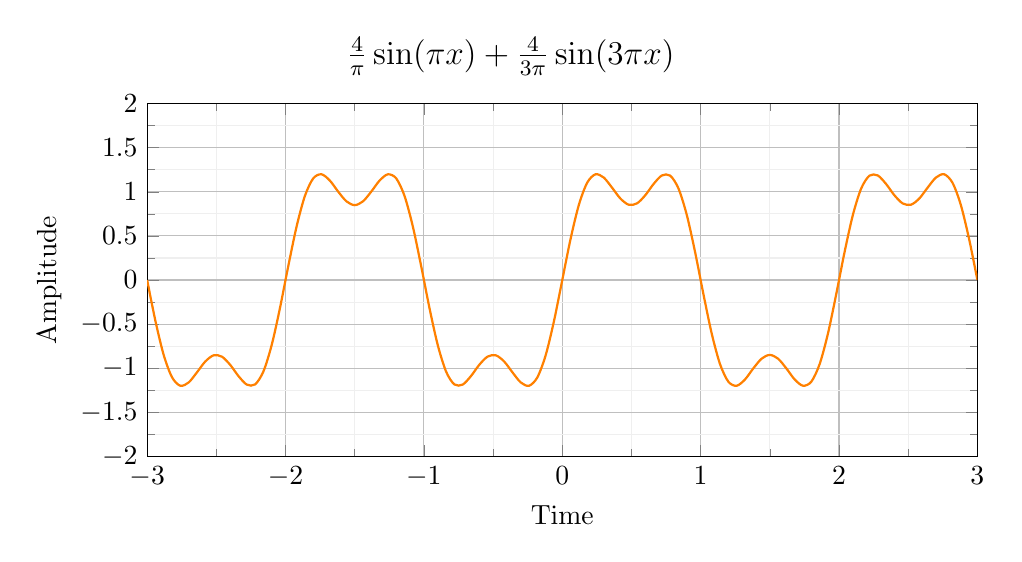
\begin{tikzpicture}
\begin{axis}[
xmin = -3, xmax = 3,
ymin = -2, ymax = 2.0,
xtick distance = 1,
ytick distance = 0.5,
grid = both,
minor tick num = 1,
major grid style = {lightgray},
minor grid style = {lightgray!25},
width = \textwidth,
height = 0.5\textwidth,
xlabel=Time,
ylabel=Amplitude,
trig format plots=rad
]
\addplot[
domain = -3:3,
samples = 101,
smooth,
thick,
orange,
] {(4 / (pi)) * sin(pi * x) + (4 / (3 * pi)) * sin(3 * pi * x)};
\end{axis}
\node[above,font=\large\bfseries] at (current bounding box.north) {$\frac{4}{\pi}\sin(\pi x)+\frac{4}{3\pi}\sin(3\pi x)$};
\end{tikzpicture}

\\\hline

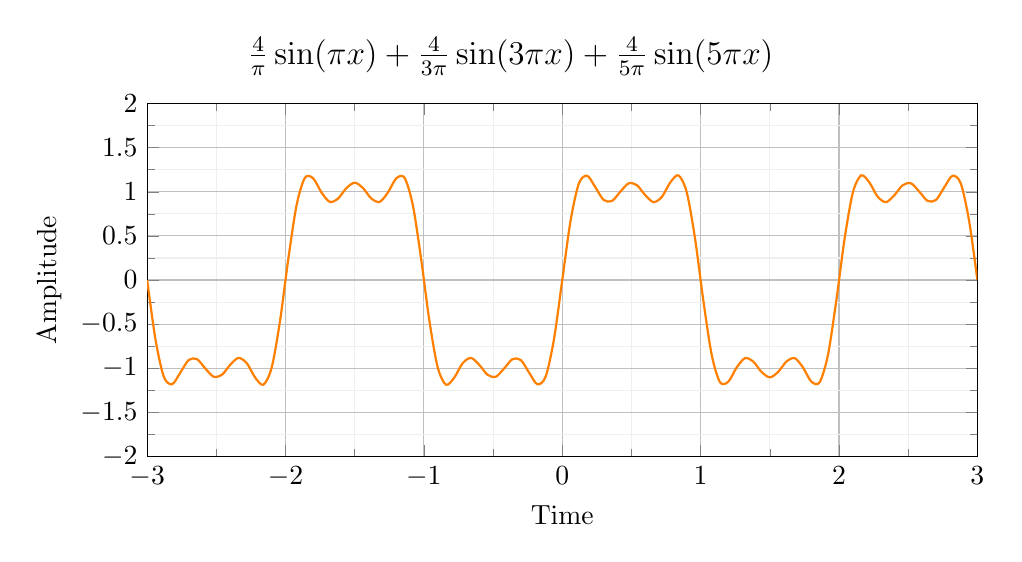
\begin{tikzpicture}
\begin{axis}[
xmin = -3, xmax = 3,
ymin = -2, ymax = 2.0,
xtick distance = 1,
ytick distance = 0.5,
grid = both,
minor tick num = 1,
major grid style = {lightgray},
minor grid style = {lightgray!25},
width = \textwidth,
height = 0.5\textwidth,
xlabel=Time,
ylabel=Amplitude,
trig format plots=rad
]
\addplot[
domain = -3:3,
samples = 101,
smooth,
thick,
orange,
] {(4 / (pi)) * sin(pi * x) + (4 / (3 * pi)) * sin(3 * pi * x) + (4 / (5 * pi)) * sin(5 * pi * x)};
\end{axis}
\node[above,font=\large\bfseries] at (current bounding box.north) {$\frac{4}{\pi}\sin(\pi x)+\frac{4}{3\pi}\sin(3\pi x)+\frac{4}{5\pi}\sin(5\pi x)$};
\end{tikzpicture}

\\\hline

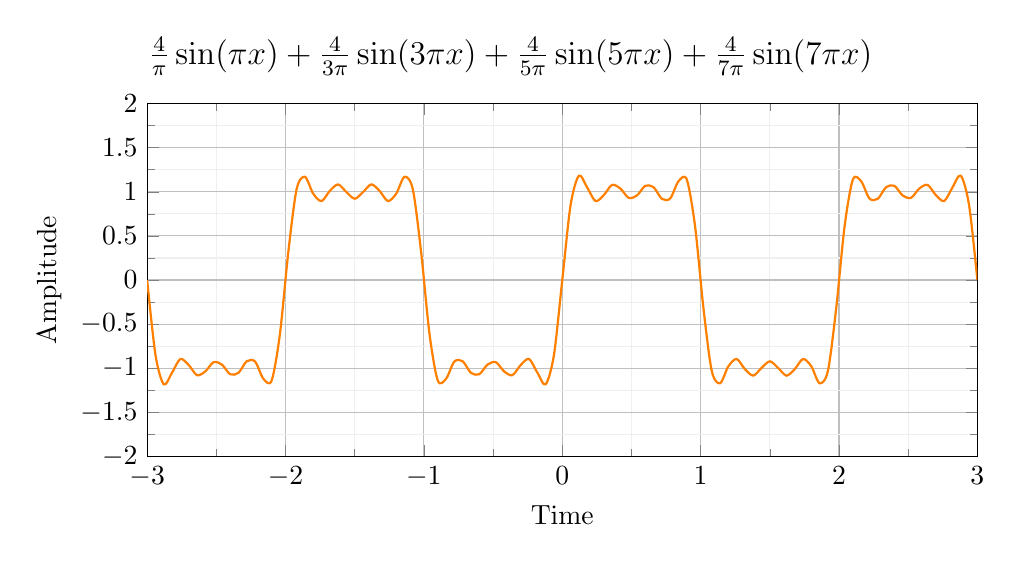
\begin{tikzpicture}
\begin{axis}[
xmin = -3, xmax = 3,
ymin = -2, ymax = 2.0,
xtick distance = 1,
ytick distance = 0.5,
grid = both,
minor tick num = 1,
major grid style = {lightgray},
minor grid style = {lightgray!25},
width = \textwidth,
height = 0.5\textwidth,
xlabel=Time,
ylabel=Amplitude,
trig format plots=rad
]
\addplot[
domain = -3:3,
samples = 101,
smooth,
thick,
orange,
] {(4 / (pi)) * sin(pi * x) + (4 / (3 * pi)) * sin(3 * pi * x) + (4 / (5 * pi)) * sin(5 * pi * x) + (4 / (7 * pi)) * sin(7 * pi * x)};
\end{axis}
\node[above,font=\large\bfseries] at (current bounding box.north) {$\frac{4}{\pi}\sin(\pi x)+\frac{4}{3\pi}\sin(3\pi x)+\frac{4}{5\pi}\sin(5\pi x)+\frac{4}{7\pi}\sin(7\pi x)$};
\end{tikzpicture}

\\\hline

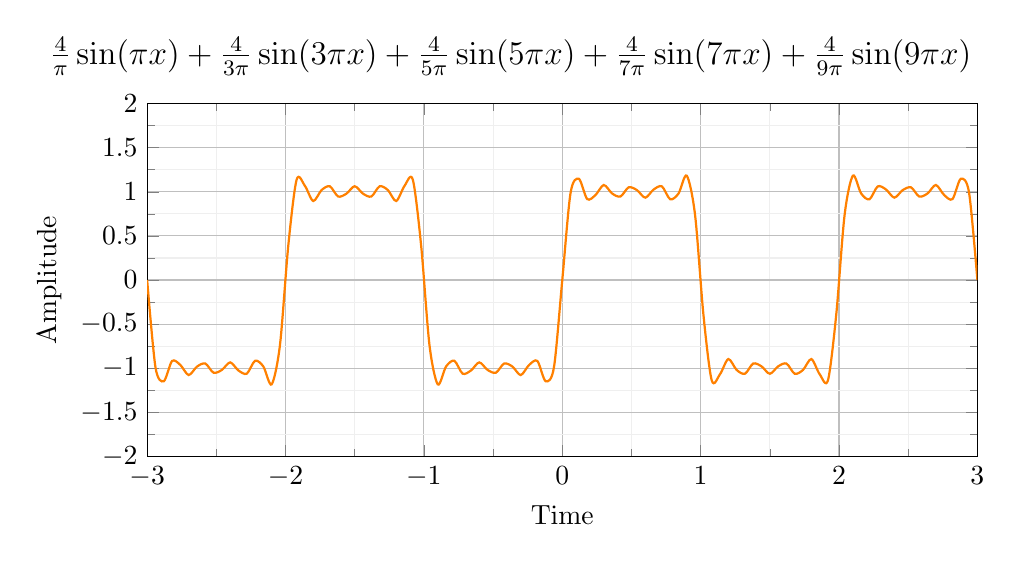
\begin{tikzpicture}
\begin{axis}[
xmin = -3, xmax = 3,
ymin = -2, ymax = 2.0,
xtick distance = 1,
ytick distance = 0.5,
grid = both,
minor tick num = 1,
major grid style = {lightgray},
minor grid style = {lightgray!25},
width = \textwidth,
height = 0.5\textwidth,
xlabel=Time,
ylabel=Amplitude,
trig format plots=rad
]
\addplot[
domain = -3:3,
samples = 101,
smooth,
thick,
orange,
] {(4 / (pi)) * sin(pi * x) + (4 / (3 * pi)) * sin(3 * pi * x) + (4 / (5 * pi)) * sin(5 * pi * x) + (4 / (7 * pi)) * sin(7 * pi * x) + (4 / (9 * pi)) * sin(9 * pi * x)};
\end{axis}
\node[above,font=\large\bfseries] at (current bounding box.north) {$\frac{4}{\pi}\sin(\pi x)+\frac{4}{3\pi}\sin(3\pi x)+\frac{4}{5\pi}\sin(5\pi x)+\frac{4}{7\pi}\sin(7\pi x)+\frac{4}{9\pi}\sin(9\pi x)$};
\end{tikzpicture}

\\\hline

\end{tabular}

\end{document}